% !TEX encoding = UTF-8
% !TEX TS-program = pdflatex
% !TEX root = ../tesi.tex

%**************************************************************
\chapter{Analisi del problema}
\label{cap:analisi-del-problema}
%**************************************************************

\intro{In questo capitolo si cercherà di dare una visione generale di cos'è un web crawler ed il dark web, inoltre, verrà descritto tramite opportune tabelle il tracciamento dei requisiti.}\\

%**************************************************************
\section{Cos'è un web crawler?}

Un web crawler è un software che analizza i contenuti di una rete in un modo metodico e automatizzato. L'utilizzo più comune dei crawler avviene sul World Wide Web; tramite una lista di url da visitare, il crawler identifica tutti i collegamenti ipertestuali presenti nel documento e li aggiunge alla lista. Data la natura della ricerca, essa potrebbe protrarsi per un tempo indefinito; tuttavia, grazie ad alcune politiche, si può influenzare l'ordine di ricerca e quali pagine evitare. I motori di ricerca odierni si basano su web crawler per poter ricercare ed indicizzare i vari siti internet.

\begin{figure}[!h] 
    \centering 
    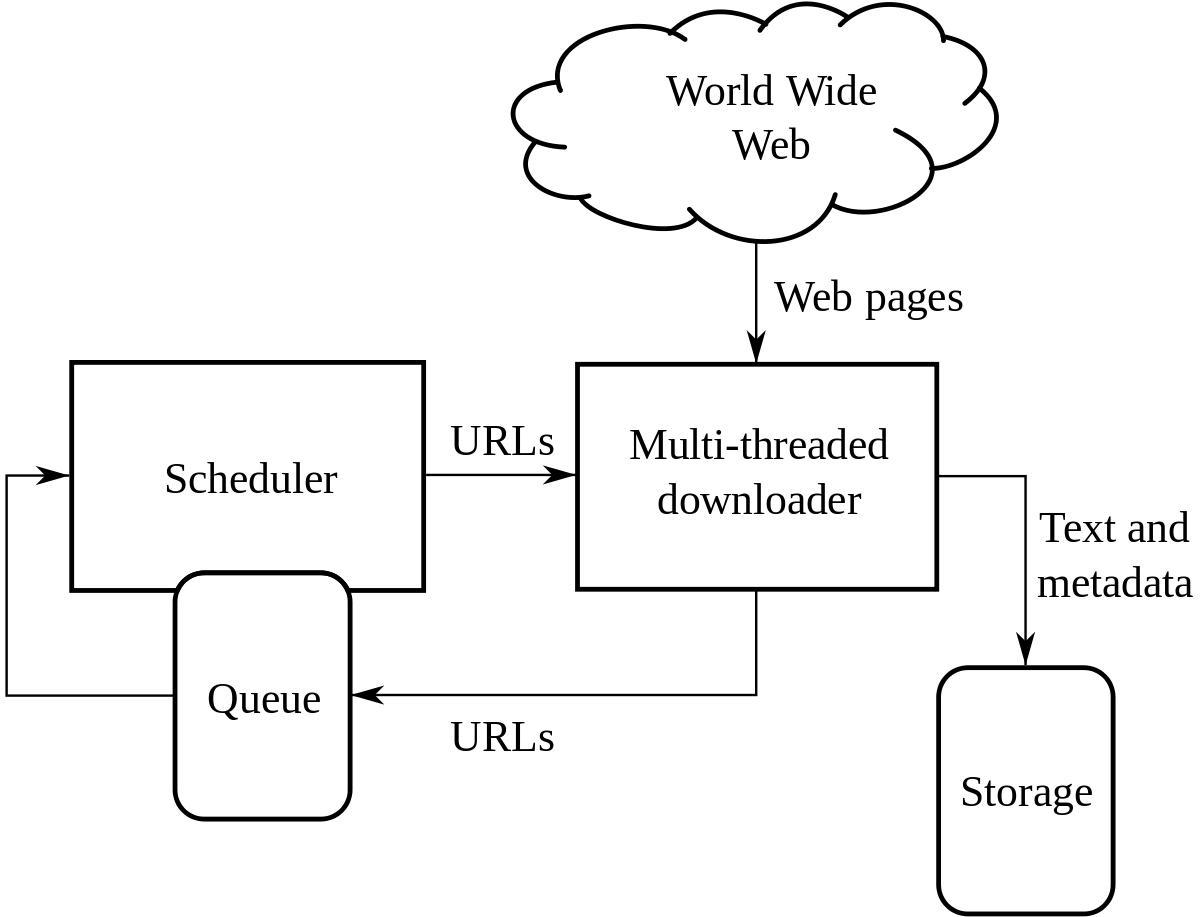
\includegraphics[width=0.5\columnwidth]{chapter2-analysis/WebCrawlerArchitecture.png} 
    \caption{Architettura di un web crawler.}
\end{figure}

%**************************************************************
\section{Cosa significa web scraping?}

Con il termine web scraping ci si riferisce all'estrapolazione di dati dai siti web. Il termine generalmente comprende anche l'estrapolazione fatta manualmente tramite software, anche se il termine principalmente si riferisce al processo automatizzato implementato tramite web crawler. L'attività principale di cui si occupa un web scraper è la trasformazione di informazioni libere in informazioni strutturate per renderle di più facile utilizzo per una successiva analisi. 

\begin{figure}[!h] 
    \centering 
    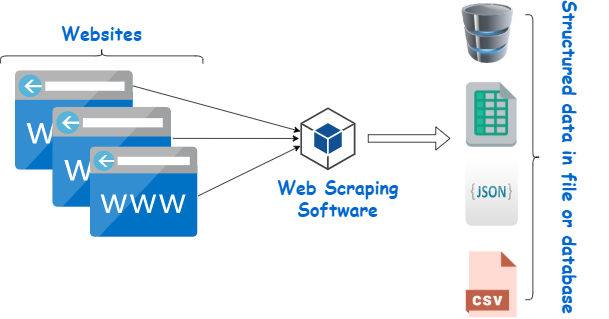
\includegraphics[width=0.6\columnwidth]{chapter2-analysis/webscraping.png} 
    \caption{Funzionamento di un web scraper.}
\end{figure}

%**************************************************************
\section{Cos'è il dark web?}
Il dark web è il World Wide Web (WWW) accessibile solamente tramite specifici software, configurazioni o autorizzazioni. Il dark web è composto da diverse reti, sia piccole reti peer-to-peer e sia grandi reti come \gls{Tor}. Le due reti utilizzate durante il progetto sono \gls{Tor} e \gls{I2P}.
%**************************************************************
\section{Studio dei moduli preesistenti}

Prima di progettare e sviluppare il nuovo modulo di web crawling, è stato necessario effettuare un’analisi della piattaforma già presente all'interno dell'azienda, per comprenderne la struttura e le funzionalità offerte. Principalmente, è stato fondamentale individuare l'organizzazione delle funzionalità di \emph{log}, dei file di configurazione e del codice. La struttura del modulo preesistente è risultata pulita, di facile comprensione e molto scalabile, richiedendo per l'inserimento del nuovo modulo l'aggiunta di poche e coincise linee di codice.

\section{Individuazione degli obiettivi}

\subsection{Notazione obiettivi}
Si farà riferimento ai requisiti secondo le seguenti notazioni:
\begin{longtable}{|p{0.2\textwidth}|p{0.8\textwidth}|}
	\caption{Notazione dei requisiti}
	\label{tab:notazione-requisiti} \\
	\hline
    \textbf{Notazione}	&	\textbf{Descrizione} \\
    OB			&	Requisiti obbligatori, vincolanti in quanto obiettivo primario richiesto dal committente. \\  
	\hline
    D			&	Requisiti desiderabili, non vincolanti o strettamente necessari, ma dal riconoscibile valore aggiunto. \\ 
	\hline
    OP			&	Requisiti opzionali, rappresentanti valore aggiunto non strettamente competitivo. \\
    \hline
\end{longtable}%

\subsection{Tabella degli obiettivi}
\begin{longtable}{|p{0.2\textwidth}|p{0.8\textwidth}|}
	\caption{Tabella degli obiettivi}
	\label{tab:tabella-obiettivi} \\
	\hline
	\textbf{Codice}	&	\textbf{Descrizione} \\
    \hline
    OB01		&	Configurazione dell'ambiente di sviluppo \\  
	\hline
    OB02		&	Scrittura del documento "Analisi dei Requisiti" \\ 
	\hline
    OB03		&	Scrittura della guida "README.md" \\
    \hline
    OB04		&	Progettazione del modulo di web crawling intelligente \\
    \hline
    OB05		&	Funzionamento del modulo su rete Tor \\
    \hline
    OB06		&	Funzionamento utilizzando la libreria "requests" \\
    \hline
    OB07		&	Implementazione di Celery \\
    \hline
    OB08		&	Configurazione dei file di log \\
    \hline
    OB09		&	Ricerca url da analizzare tramite tag href \\
    \hline
    OB10		&	Implementazione della ricerca di informazioni interessanti tramite regex \\
    \hline
    OB11		&	Implementazione di priorità di analisi calcolate dinamicamente ed intelligentemente \\
    \hline
    OB12		&	Implementazione di un sistema per riprovare url con i quali è fallita la connessione \\
    \hline
    D01			&	Funzionamento del modulo su clear web \\
    \hline
    D02			&	Implementazione di un sistema di caching tramite redis degli url visitati \\
    \hline
    D03			&	Ricerca url da analizzare in tutto il codice sorgente della pagina \\
    \hline
    D04			&	Sanitizzazione degli url estrapolati \\
    \hline
    D05			&	Implementazione di una lista di siti di cui evitare l'analisi \\
    \hline 
    D06			&	Implementazione dell'utilizzo di Selenium \\
    \hline
    D07			&	Creazione di file di log in formato csv \\
    \hline
    D08			&	Implementazione di chiamate di rete intelligenti tramite gli headers HTTP \\
    \hline
    D09			&	Salvataggio ed utilizzo dei cookie di sessione \\
    \hline
    D10			&	Creazione dell'ambiente di test \\
    \hline
    OP01		&	Implementazione di molteplici browser tramite selenium \\
    \hline
    OP02		&	Funzionamento del modulo su rete I2P \\
    \hline
    OP03		&	Estensiva gestione delle eccezioni \\
    \hline
    OP04		&	Implementazione del salvataggio di file su directory temporanee \\
    \hline
    OP05		&	Salvataggio di screenshot e codice sorgente degli url interessanti su Amazon S3 \\
    \hline
    OP06		&	Scrittura dei test di unità \\
    \hline
\end{longtable}%

%**************************************************************
\section{Caratteristiche del modulo}
%**************************************************************

Il modulo, oltre a fornire tutte le funzionalità descritte precedentemente, deve avere le
seguenti caratteristiche: deve essere scalabile e performante, per permettere un aumento o diminuzione delle risorse; questo viene realizzato tramite una corretta progettazione, mirata alla ottimizzazione dell'utilizzo di memoria, per poter permettere a più istanze del programma di essere eseguite contemporaneamente tramite la libreria \emph{Celery}.